%!TEX root = ../thesis.tex
%*******************************************************************************
%****************************** Second Chapter *********************************
%*******************************************************************************

\chapter{Background}

\ifpdf
    \graphicspath{{Chapter2/Figs/Raster/}{Chapter2/Figs/PDF/}{Chapter2/Figs/}}
\else
    \graphicspath{{Chapter2/Figs/Vector/}{Chapter2/Figs/}}
\fi

\section{Introduction}

In this section, I will introduce the components required for the rest of this thesis.

% AWF: I want to use a term which encompasses model fitting & deep learning parameter prediction. 

\section{Model fitting}
    Model (or mesh) fitting encompasses a set of methods that work by adapting a 3D template mesh to either an input image or input video sequence. Such techniques therefore return a full 3D model intended to faithfully reconstruct the performance given by the tracking target, although the accuracy of this reconstruction is heavily conditioned on the quality of the method.
    

    \subsection{Form of the template prior}
    A polygon mesh $M = (V, T)$ is a collection of vertices, edges bound by vertex pairs, and polygons bound by sequences of edges and vertices~\cite{smith2006vertex}. Although other convex shapes are allowed, mesh polygons will always be considered triangular (and hence referred to as \emph{triangles}) unless explicitly stated otherwise. An example mesh is shown in Figure~\ref{fig:polygon_mesh}. 
    
    \begin{figure}[H] % Example image
        \center{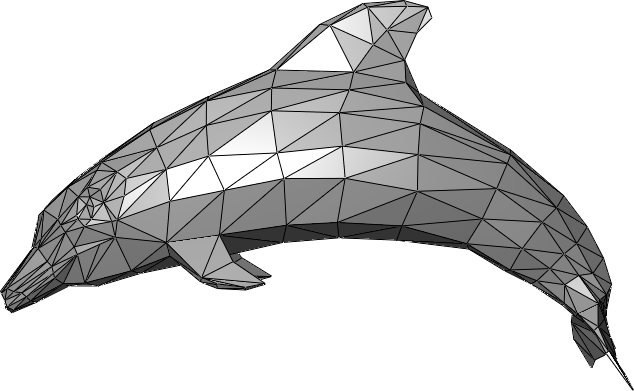
\includegraphics[width=0.5\linewidth]{dolphin_mesh}}
        \caption{A polygon mesh~\cite{polygon_mesh}.}
        \label{fig:polygon_mesh}
    \end{figure}

    
    \subsection{Mesh deformation}
    The process of adapting a 3D mesh is known as \textit{mesh deformation} and is common across many computer graphics applications, particuarly those in which models are designed to represent dynamic objects. To constrain an optimization function (or simplify the animation process), it is useful to introduce priors that prevent unnatural mesh movement. Two methods for achieving this are discussed:

        \subsubsection{Skeletal Rigging and Linear Blend Skinning}
        In cases that the mesh shape is known in advance, it is common to follow a process known as \textit{rigging}, in which the mesh is augmented with a hierarchical bone structure. The point at which two bones meet is called a \emph{joint}, and these can be used to define acceptable centres of rotation for mesh deformation. It is possible to describe a distribution of joint configurations, which could be used to constrain the mesh to (in the case of human / animal subjects) anatomically achievable poses. It is also simple to define conceptual `body parts' from a rigged mesh, by considering regions between pairs of joints; for example a lower leg region can be defined between a knee and ankle joint. A simple example of a rigged 2D mesh with joints indicated by green diamonds is shown in Figure~\ref{fig:finger_model}. Note how the mesh surface deforms naturally as the joints are displaced.
        
        \begin{figure}[H]
            \centering
            \begin{subfigure}{0.48\linewidth}
            \centering
                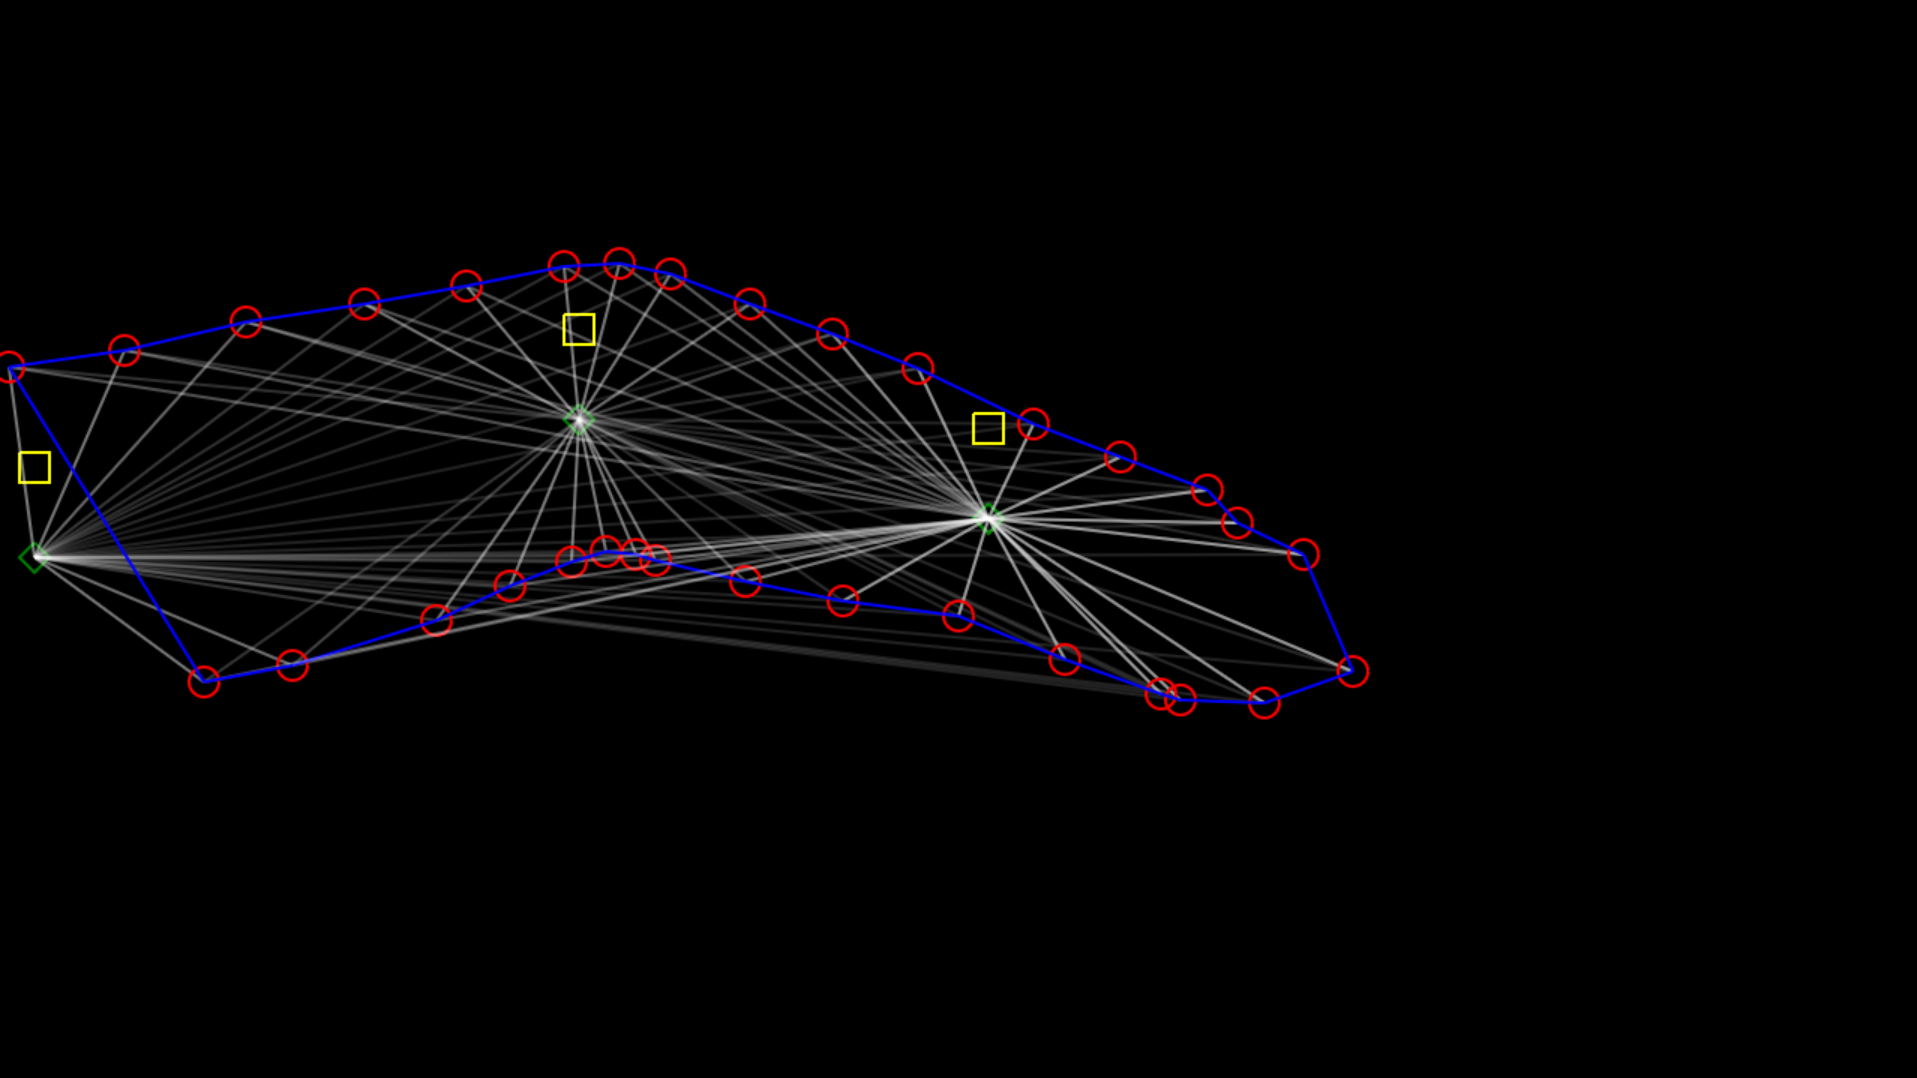
\includegraphics[width=1\linewidth]{finger/finger1}
                \caption{Default joint positions.}
            \end{subfigure}
            \begin{subfigure}{0.48\linewidth}
            \centering
                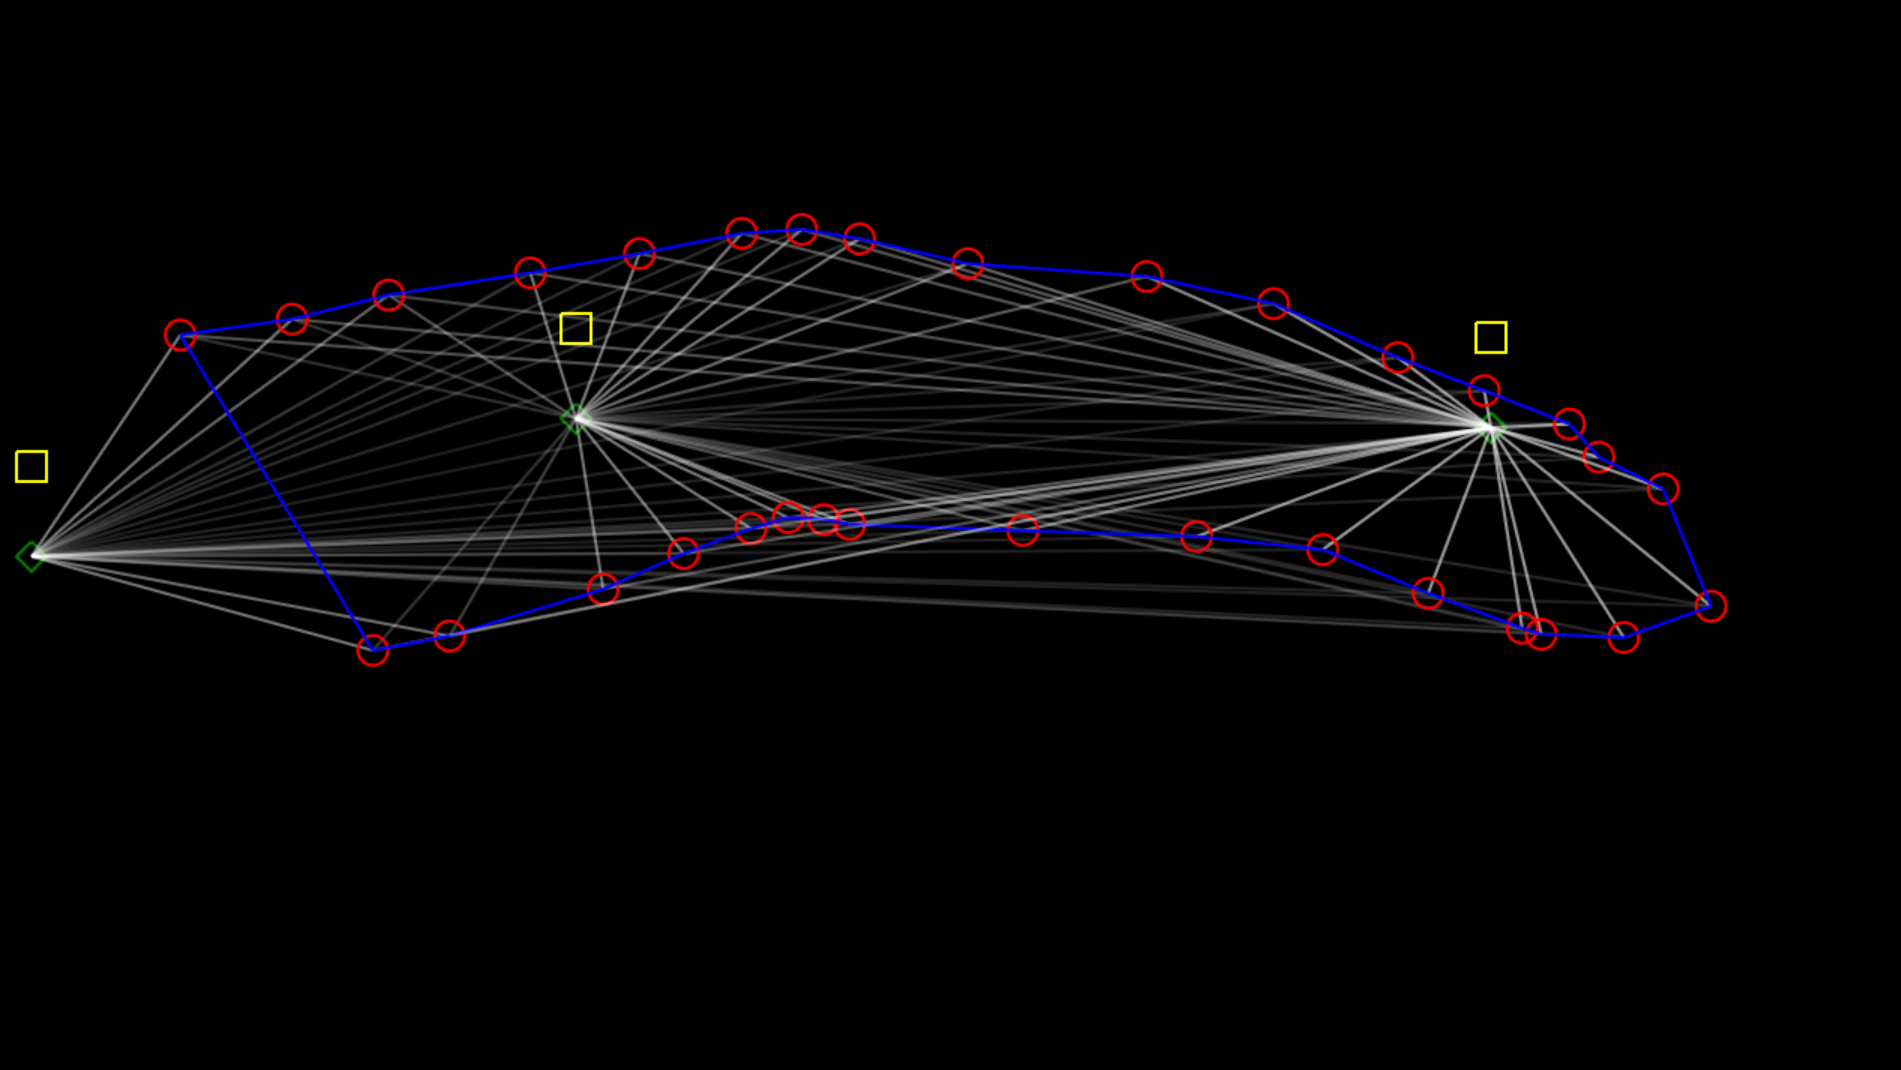
\includegraphics[width=1\linewidth]{finger/finger2}
                \caption{Right-most joint displaced.}
            \end{subfigure}
            \begin{subfigure}{0.48\linewidth}
            \centering
                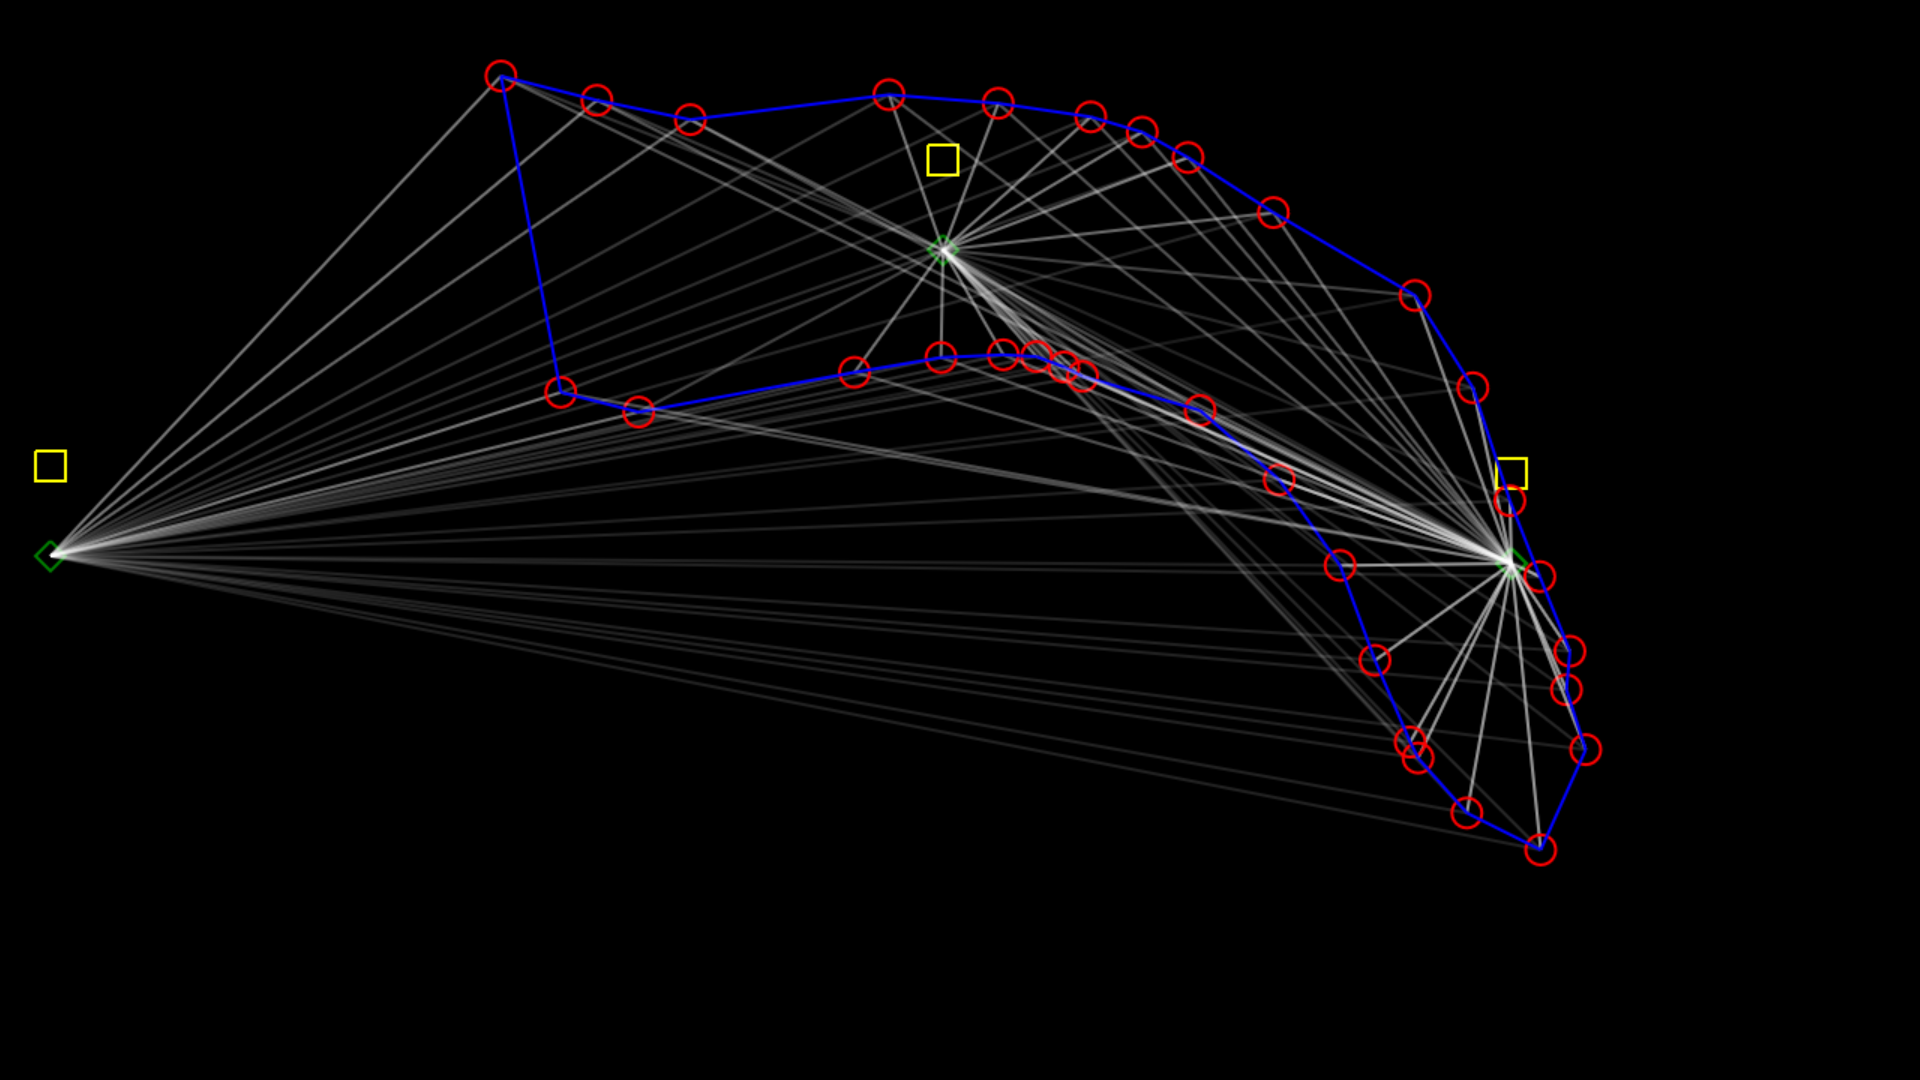
\includegraphics[width=1\linewidth]{finger/finger3}
                \caption{Central joint displaced and right-most joint displaced and rotated.}
            \end{subfigure}%
            \caption{Web application demonstrating LBS on a 2D finger mesh. Joints are denoted as green diamonds.}
            \label{fig:finger_model}
        \end{figure}

        \clearpage
        Formally, a skinned mesh consists of a set of rigged vertices $V \subseteq \mathbb{R}^3 \times \mathbb{R}^{|J|}$, a set of faces $F \subseteq V^3$ and joints $J \subseteq R^{3\times3}$. Each vertex $v = (x, s) \in V$ consists of positional coordinate $x \in \mathbb{R}^{3}$ and a weight vector $s \in \mathbb{R}^{|J|}$ which describes the level of influence each joint $j \in J$ has over its movement. Many approaches exist for assigning weights, but perhaps the simplest is to build a vector with entries corresponding to the distance from the vertex to each joint centre. Skinning weight vectors are normalized such that their entries sum to one, and for computational reasons, the number of non-zero elements is typically limited to 2 or 4. The weakness of such models is that artifacts and other unrealistic deformations can occur around the model joints, particularly for meshes that model non-linear structures such as humans. However, the technique is frequently used in computer graphics and game design when a character's shape is known ahead of time.

        To assist in explanation, Figure \ref{fig:rigged_cylinder} shows skinning weight influences from three joints within a rigged cylinder mesh. Here, $|J| = 3$ and each vertex $v_{i} = (x_{i}, s_{i}) \in V$ has a skinning weight vector $s_{i} \in \mathbb{R}^{3}$. Each model joint is assigned a distinct RGB value, shown separately in (a), (b) and (c), and together in (d) by linearly combining the colours. This linear blend colorization scheme will be frequently used in later sections of this report.

        \begin{figure}[H]
            \centering
            \begin{subfigure}{0.25\linewidth}
            \centering
                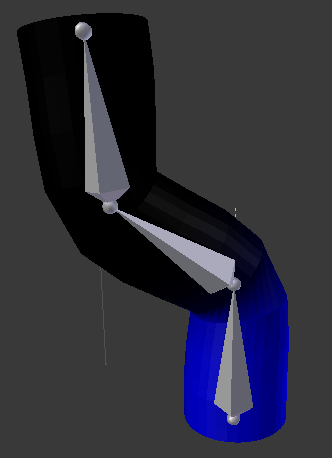
\includegraphics[width=1\linewidth]{wonky_pole/lower_bone}
                \caption{Lower joint.}
            \end{subfigure}%
            \begin{subfigure}{0.25\linewidth}
            \centering
                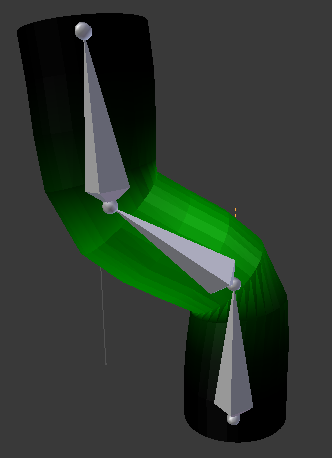
\includegraphics[width=1\linewidth]{wonky_pole/middle_bone}
                \caption{Middle joint.}
            \end{subfigure}%
            \begin{subfigure}{0.25\linewidth}
            \centering
                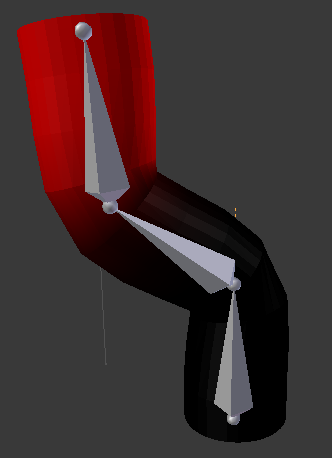
\includegraphics[width=1\linewidth]{wonky_pole/upper_bone}
                \caption{Upper joint.}
            \end{subfigure}%
            \begin{subfigure}{0.25\linewidth}
            \centering
                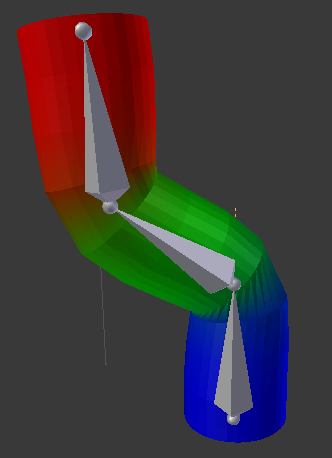
\includegraphics[width=1\linewidth]{wonky_pole/linear_blend}
                \caption{Linear blend.}
            \end{subfigure}%
            \caption{A rigged cylinder with $|J| = 3$ and where each vertex $v_{i} = (x_{i}, s_{i}) \in V$ has a skinning weight vector $s_{i} \in \mathbb{R}^{3}$.}
            \label{fig:rigged_cylinder}
        \end{figure}

        Figure \ref{fig:rigged_quadruped} shows a more complex rigged quadruped mesh with $|J| = 25$ with skinning weight influences again shown by the linear blend colorization scheme. Again, each joint is assigned a unique RGB value and a vertex's colour is calculated by linearly combining joint colours with skinning weight vectors given by the $\{s_{i}\}$. A triangle's colour is then generated by averaging the colours given for the three surrounding vertices.

        \begin{figure}[H] % Example image
            \center{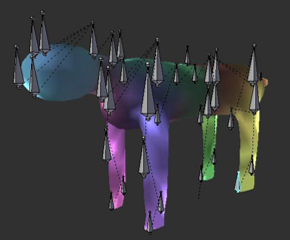
\includegraphics[width=0.5\linewidth]{linear_blend_bold_bones}}
            \caption{A rigged quadruped with $|J| = 25$ and where each vertex $v_{i} = (x_{i}, s_{i}) \in V$ has a skinning weight vector $s_{i} \in \mathbb{R}^{3}$. Visualization uses the linear blend colorization scheme in which each joint is assigned a unique RGB value.}
            \label{fig:rigged_quadruped}
        \end{figure}

        Once a mesh has been suitably rigged, there are a number of options (e.g. Linear Blend Skinning (LBS), Dual Quaternions~\cite{kavan2007skinning} etc.) for applying a particular mesh deformation. Typically, a user assigns a transformation (in this case comprising a rotation and transformation) to each `joint' and the updated positions $\bar{x_{i}}$ of the remaining vertices $v_{i}$ with original positions $x_{i}$ are then calculated. The original transformation for each joint (i.e. before the deformation) is expressed as a matrix $U_{j}$. The transformation after the deformation has been applied is captured by $D_{j}$. Note that $s_{ij}$ denotes the skinning weight influence of joint~$j \in J$ on vertex $v_{i} \in V$.
        
        The updated positions $\bar{x_{i}}$ can then be calculated by LBS:

        \begin{equation}
            \bar{x_{i}} = \sum_{j=1}^{|J|}s_{ij}D_{j}U_{j}^{-1}x_{i}
        \end{equation}

        \clearpage
        \subsubsection{Rendering}
        The process of generating a 2D image from a 3D polygon mesh is known as rendering and can be achieved through a process known as raytracing. Raytracing is a rendering technique able to generate photorealistic 2D images from the scene. It can be considered the opposite process by which the human eye perceives the world, as this method involves lines being cast outwards, beginning at a point known as the \emph{camera origin}. Figure \ref{fig:raycasting} shows a typical set up, in which rays are cast from the camera origin through each pixel on the image plane. The colour for the pixel is obtained by following the ray through the scene until a light source or non-reflective surface is reached, taking into account any reflections or non-opaque scene items. Due to the considerable comptuation required, the operation is often parallelized and assigned to the GPU. However, the technique is typically considered unsuitable for real-time rendering of complex scenes (due to complex ray paths) or when high resolution images (many rays required) are needed. However, for this work, scenes are typically made up of a single non-reflective, solid mesh surface and contain no complex elements (e.g.\ shadows, non-constant lighting.

        \begin{figure}[H] % Example image
            \center{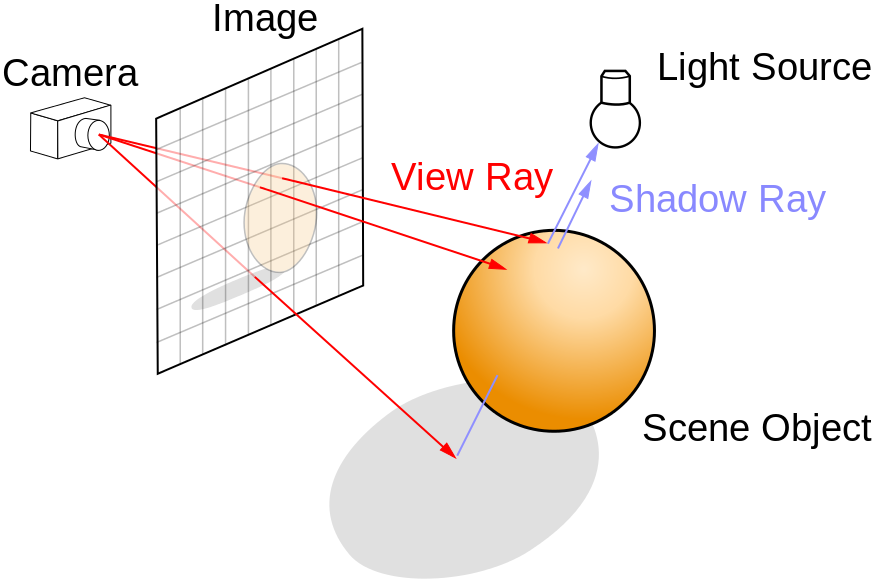
\includegraphics[width=0.5\linewidth]{ray_trace}}
            \caption{Diagram showing raycast rendering.~\cite{rendering}.}
            \label{fig:raycasting}
        \end{figure}

        It is also worth noting that the standard method for raycasting is not differentiable, causing problems for differentiable optimizers (including neural networks). However, alternative rendering methods~\cite{loper2014opendr} are available for these purposes.


\section{Methods for model fitting}
The following section describes an number of existing model fitting methods.

\subsection{Fitting a rigged template mesh to a set of correspondences}
 % Edit to talk about e.g. SMPLify

%  Model fitting algorithms are typically provided with point correspondences between the template mesh and input images in order to help constrain the optimization. Correspondences are either provided by a human annotator or predicted by a discriminative machine learning model.

Taylor et al. demonstrate a model fitting approach that operates on a rigged 3D human mesh~\cite{taylor2012vitruvian}. Their aim is to learn a set of pose parameters $\theta \in \mathbb{R}^{d}$ so as to explain a set of image points $D = \{x_{i}\}_{i=0}^{n}$. Data points $x_{i} \in \mathbb{R}^{3}$ are collected from a calibrated depth camera. Once these pose parameters are learnt, the mesh is deformed according to the LBS algorithm defined above.

The template mesh contains $|J| = 13$ joints, and $m$ skinned vertices ${V} = \{v_{i}\}_{i=1}^{m}$. Again, each vertex $v_{i} \in V$ is defined as:

\begin{equation}
    v_{i} = (x_{i}, s_{i})
\end{equation}
where $x_{i} \in \mathbb{R}^{3}$ represents the base 3D vertex positions in a canonical pose $\theta_{0}$ and the $s_{i} \in \mathbb{R}^{|J|}$ are skinning weight vectors. It is possible to define a mesh induced by a pose $S(\theta) = (V, T)$ for vertices $V$ and triangles $T$. Due to the resemblance of the mesh surface induced by the canonical mesh pose $\theta_{0}$ and Da Vinci's Vitruvian man~\cite{davinci}, this surface is referred to as the \emph{Vitruvian Manifold}, and is shown in Figure~\ref{fig:vitruvian_man}. 

\begin{figure}[H] % Example image
    \center{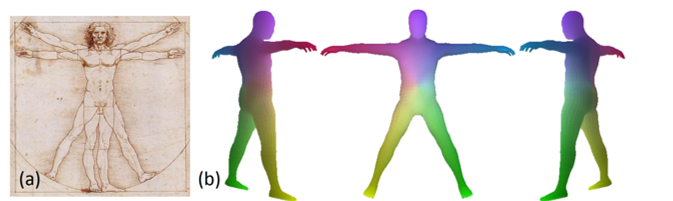
\includegraphics[width=0.95\linewidth]{vitruvian_man}}
    \caption{(a) Vitruvian Man by Leonardo da Vinci~\cite{davinci} and (b) the Vitruvian Manifold reprinted from~\cite{taylor2012vitruvian}.}
    \label{fig:vitruvian_man}
\end{figure}

The primary contribution of this paper is the design of a model able to predict \emph{dense correspondences} between the 3D canonical mesh and input 3D images. In other words, \emph{every} body pixel on an input image is regressed to a point on the vitruvian manifold mesh. The authors demonstrate the accuracy of these correspondences is sufficient for \emph{one-shot learning}, meaning there is no need to recalculate correspondences after a subsequent optimization step. The reason for this is the strength of the core error term which penalizes the sum of errors between image points $\{x_{i}\}_{i=0}^{n}$ and determined mesh correspondences $U = \{u_{i}\}_{i=0}^{n} \subseteq V$:

\begin{equation}
    E_{\text{data}}(\theta,U) =\sum_{i=1}^{n}s_{i} \cdot d(x_{i}, M(u_{i}; \theta))
\end{equation}
where $M(u_{i}, \theta)$ is the position of vertex $u_{i}$ on the vitruvian manifold mesh after having been displaced by an LBS deformation with respect to the pose~$\theta$. 

The sheer quantity of correspondences greatly constrain their optimizer which works well, even on challenging input images. Much of this report focuses on how this paper can be extended to work for animal subjects, incorporating deep learning correspondence prediction and working from monocular RGB input data.

\subsection{Model fitting with deep learning}

This is how you do this using a deep network. 



